\section{Discussion}
\label{sec:discuss}

Even though we have a decent success rate for most images there are some particular failure modes that are worht talking about.

\subsection{Fewer Edges}
The first such scenario is where the edges of the item are simply difficult to detect.
In figure~\ref{fig:missedEdge} the Canny edge detector is unable to find the right edge of the paper.
This kind of error could be adressed potentially with more pre-processing of the image.
There is a tradeoff with this type of error and some of the future errors which are results of having too many edges.
If we have the edge detector identify more edges it becomes difficult to pick the right set.

\begin{figure}[t]
\begin{center}
   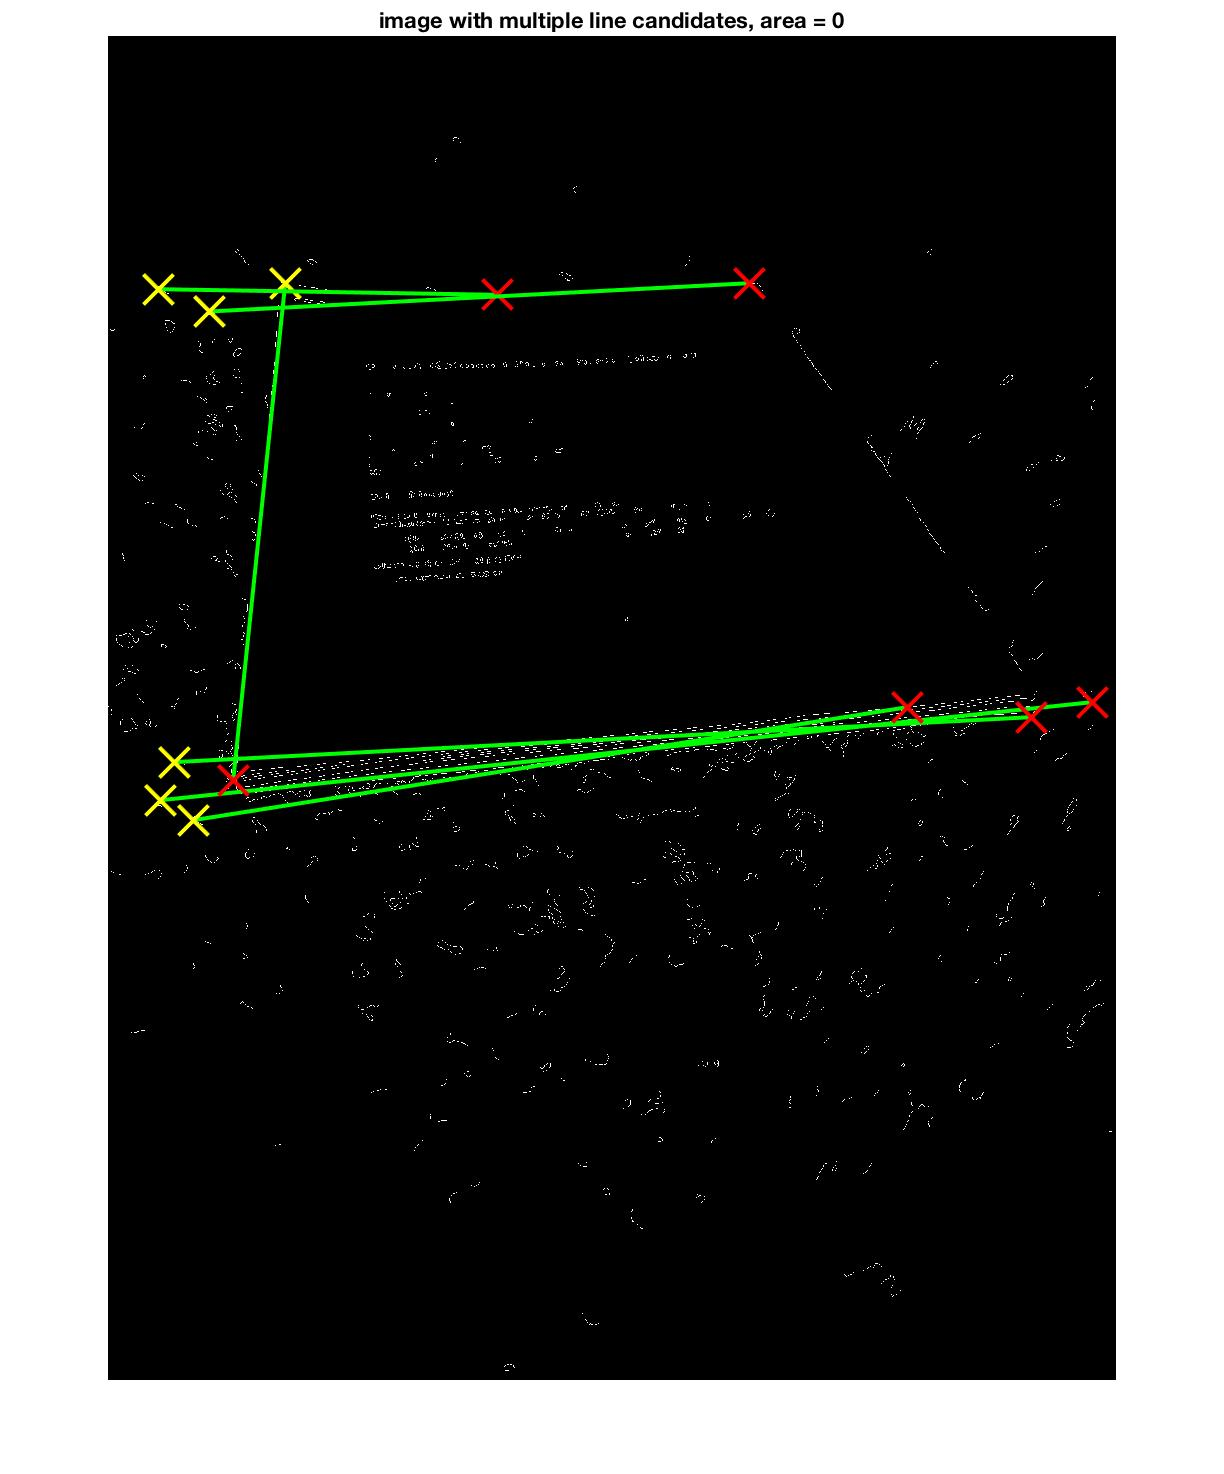
\includegraphics[width=0.8\linewidth]{figures/missedEdge.jpg}
\end{center}
\caption{An image which has an undetectable edge.}
\label{fig:missedEdge}
\end{figure}


\subsection{Extra Edges}
The remaining types of errors fall into a different category where we have detected edges that do not correspond to the actual edges of the book cover.

The first failure mode we see is where the book has significant depth that also has a sharp edge with the background as in figure~\ref{fig:depthError}.
This causes the largest bounding box to include an additional edge of the book that is not the true edge of the cover.
One heuristic to possibly detect the difference between the cover and the side of the book would be to expect that side of the book will often be a consistent cover, e.g. white.
Then if we find that we have two quadrilaterals to pick from and one of them is essentially the other but with a large monochrome segement attached we can guess that this is the side of the book.


\begin{figure}[t]
\begin{center}
   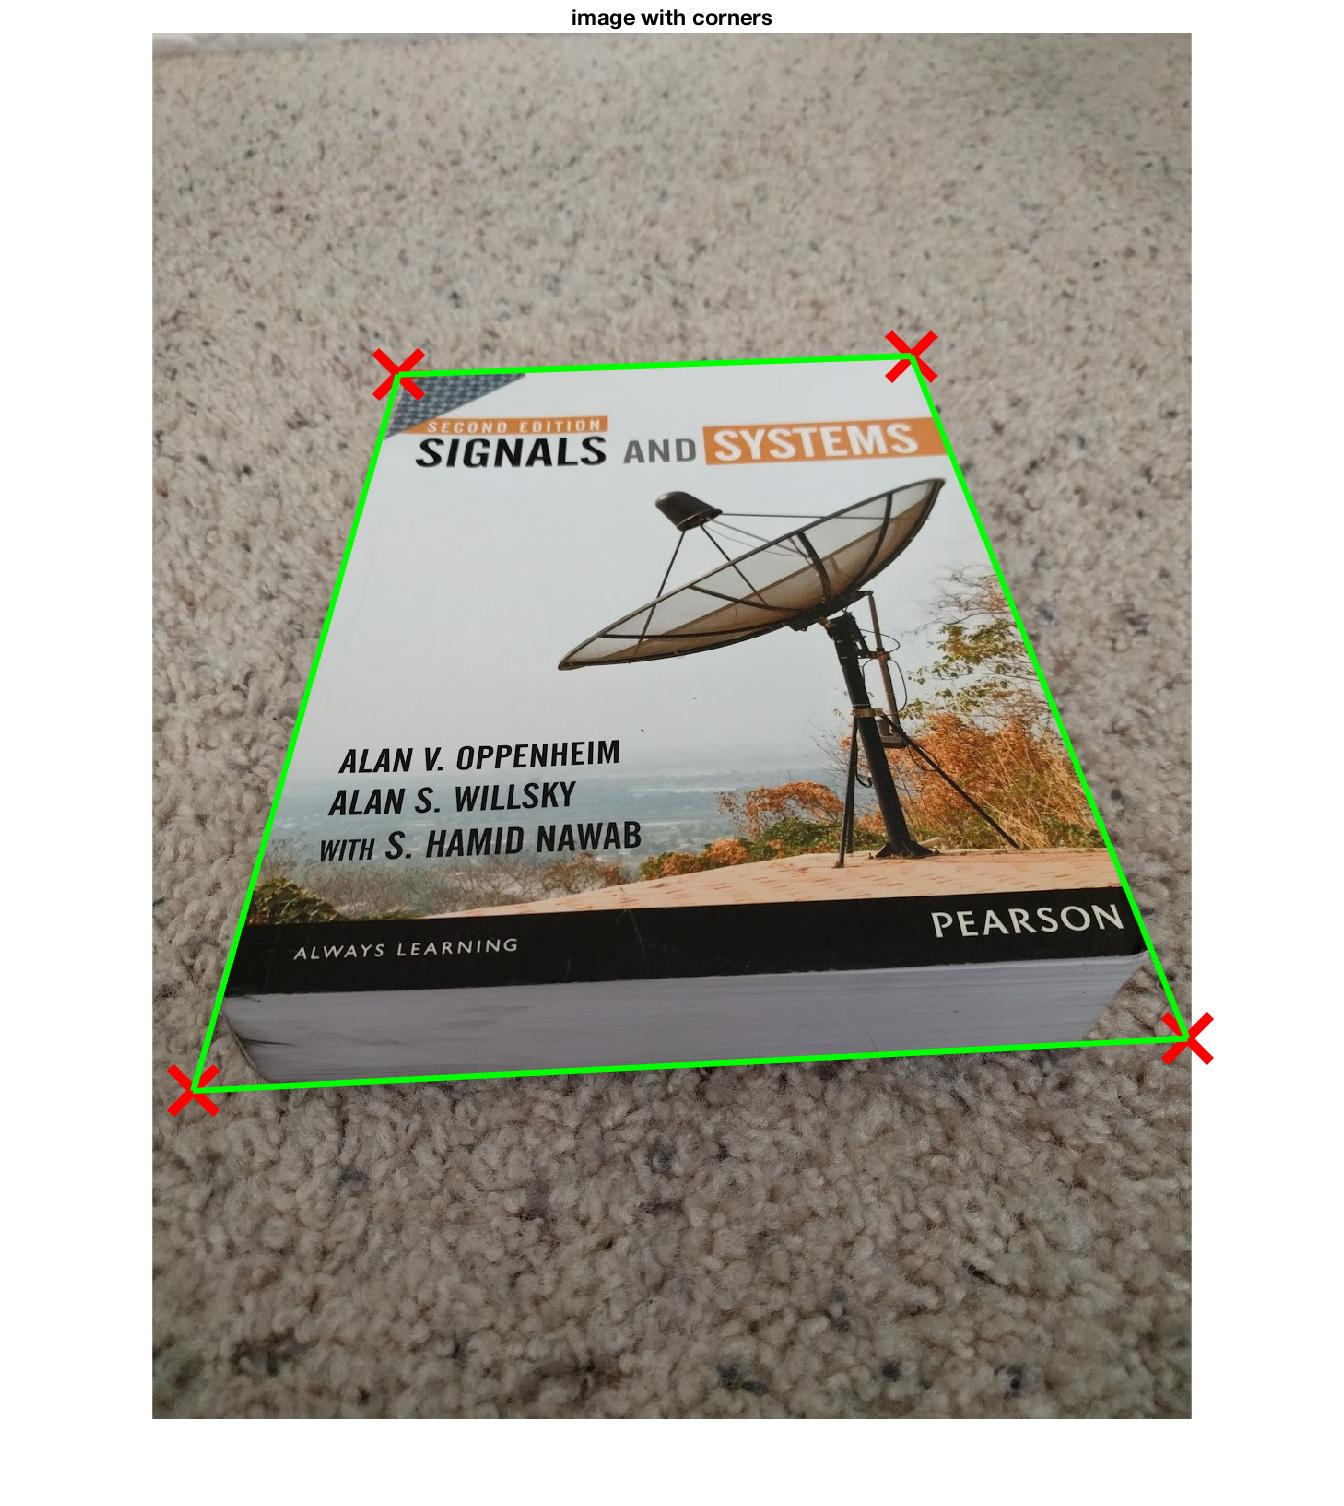
\includegraphics[width=0.8\linewidth]{figures/depthError.jpg}
\end{center}
\caption{A book which is deep and thus has a larger rectangle than the correct one.}
\label{fig:depthError}
\end{figure}

A similar failure mode appears in figure~\ref{fig:shadowError}.
However in this failure rather than the side of the book it is the shadow of the book that creates the larger false rectangle.
This failure seems similar enought to the previous mode that the same heuristic may work well again.
If the shadow is solid enough to be detected as an additional line then it is probably monochrome just like the side of the book.
In our example image this turns out to be true and so we hypothesize that using the same monochrome attachement heurstic from before could correct this image.

\begin{figure}[t]
\begin{center}
   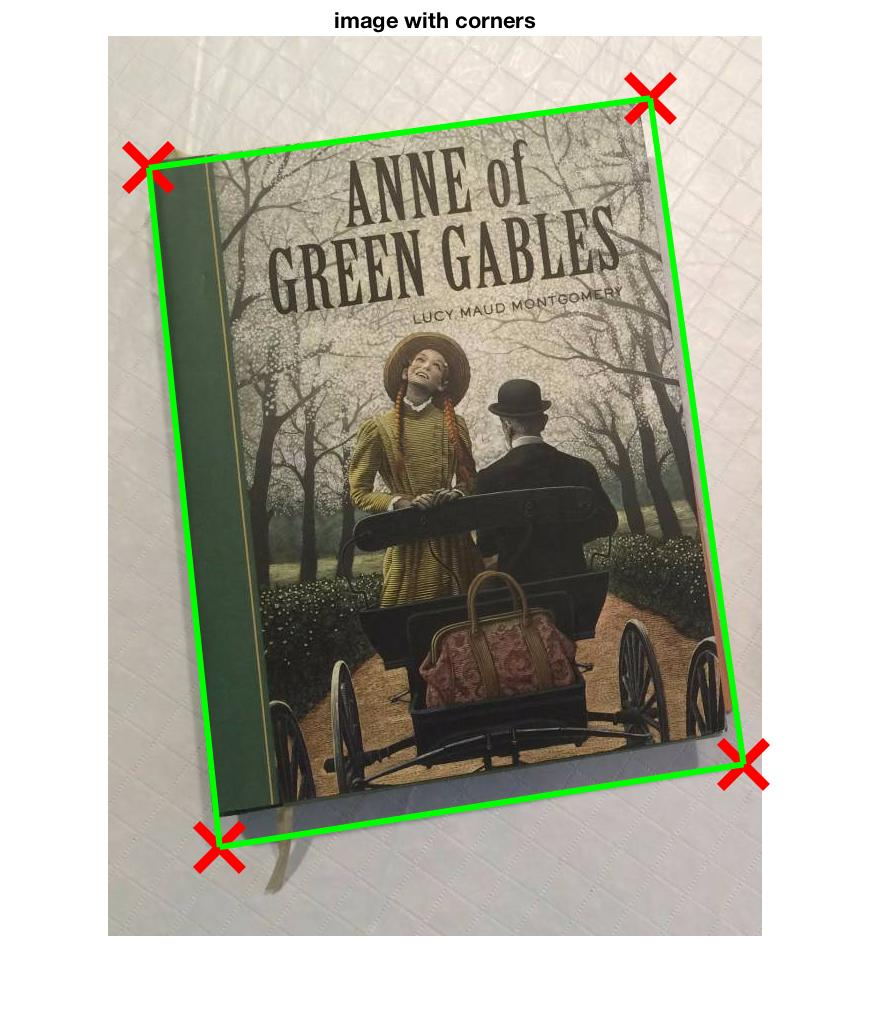
\includegraphics[width=0.8\linewidth]{figures/shadowError.jpg}
\end{center}
\caption{A book which has a well defined shadow and thus a larger rectangle than the correct one.}
\label{fig:shadowError}
\end{figure}

Finally the last failure mode we discuss is that of extra lines on the cover of the book or page.
These are actual lines that should be detected by any sensible edge detector but cause problems with our bounding box selection as seen in figure~\ref{fig:extraEdges}.
This is certainly our most difficult to handle failure mode, and has no clear solution of mitigation technique.

\begin{figure}[t]
\begin{center}
   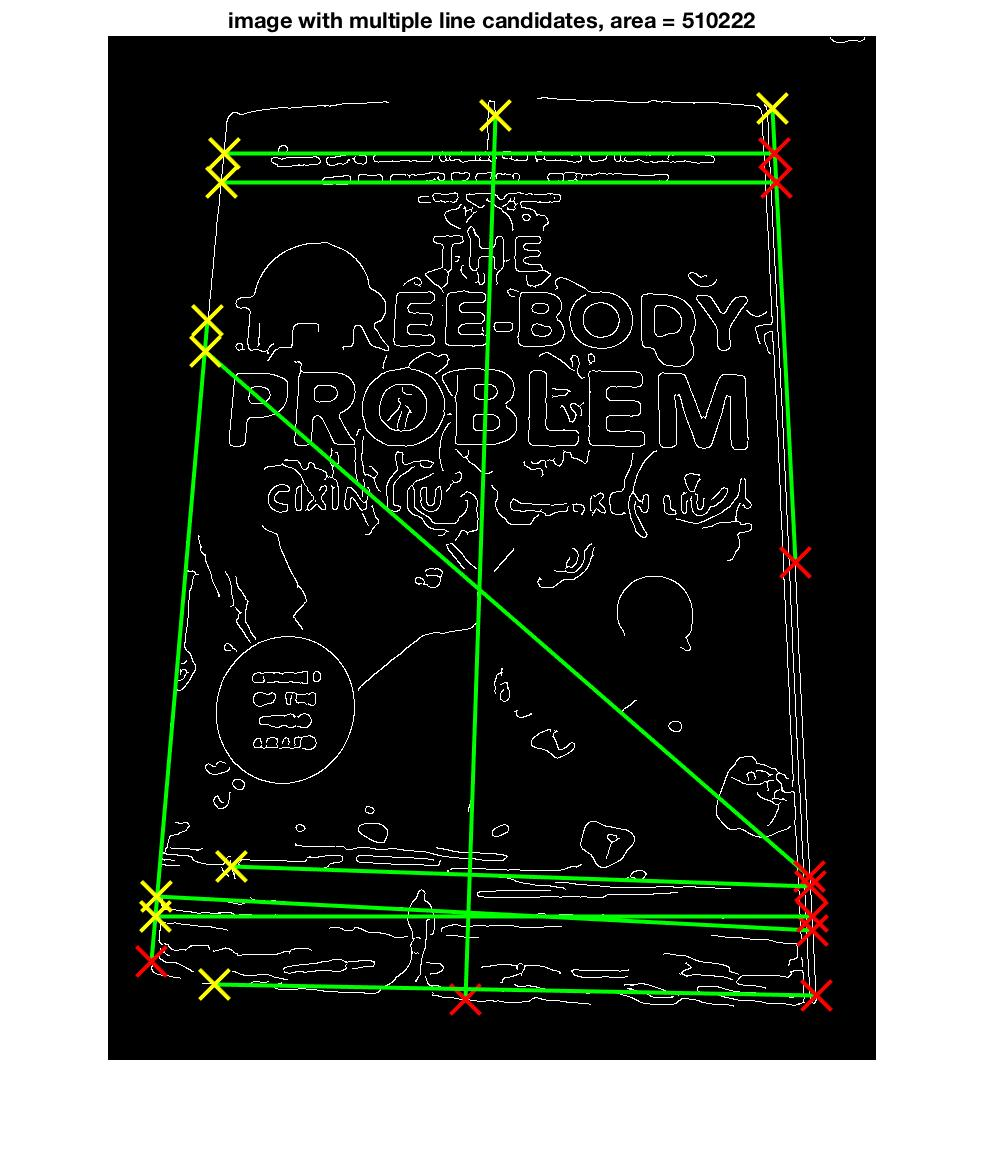
\includegraphics[width=0.8\linewidth]{figures/extraEdges.jpg}
\end{center}
\caption{A book which has a lot of extra edges on the cover making it hard to find the right set of four.}
\label{fig:extraEdges}
\end{figure}
